\documentclass[10pt]{article}
\usepackage[T1]{fontenc}
\usepackage[utf8]{inputenc}
\usepackage[nottoc]{tocbibind}
\usepackage{graphicx}
\usepackage{subcaption}
\usepackage{indentfirst}
\usepackage[a4paper, margin=0.8in]{geometry}
\usepackage{hyperref}
\usepackage{float}
\usepackage[polish]{babel}
\usepackage[sorting=none]{biblatex}
\usepackage{csquotes}
\usepackage{amsfonts}
\usepackage{amsmath}
\usepackage{url}
\usepackage{tabularx}
\renewcommand{\arraystretch}{1.5}


%\graphicspath{{./images/}}
\addbibresource{bibliography.bib}

\title{Zastosowanie \textit{Monte Carlo Tree Search} \\
oraz \textit{Upper Confidence Bound Applied To Trees} \\
do stworzenia sztucznej inteligencji grającej w grę Othello\\
\large{Raport}}
\author{Szymon Stasiak \and Przemysław Woźniakowski}
\date{\today}

\begin{document}

\maketitle
\begin{abstract}
    Monte Carlo Tree Search to potężna metoda, która znalazła zastosowanie w wielu dziedzinach sztucznej inteligencji. Szczególnie interesującym tematem, jest zastosowanie jej w obszarze gier dwuosobowych, gdzie popularna jest wersja równoważąca eksploatacje z eksploracją za pomocą metody Upper Confidence Bound 1 applied to trees. W ramach projektu stworzona została implementacja metody Monte Carlo Tree Search wykorzystującej metodę UCT dla gry Othello. Dodatkowo zaimplementowane zostało także podejście bazujące na algorytmie \textit{alpha-beta pruning}, oraz dwie modyfikacje UCT: podejście UCB1-tuned oraz podejście, w którym powtarzające się w drzewie stany, były łączone we wspólny węzeł. W ramach testów przeprowadzona została seria pojedynków wszystkich algorytmów w formacie każdy z każdym. Wbrew wstępnym oczekiwaniom, najlepiej wypadła w nich podstawowa wersja algorytmu UCT, natomiast wersja heurystyczna zgodnie z oczekiwaniami zajęła ostatnie miejsce. Wszystkie wersje UCT wykonywały ruchy z podobnym czasem, choć nieznacznie szybsza była wersja z grupowaniem ruchów. Kolejnym testem było przeciwstawienie algorytmów średnio-zaawansowanemu, prawdziwemu graczowi w serii 3 gier \textit{Best of 3}, czyli do 2 zwycięstw. W tych pojedynkach również najlepsza okazała się podstawowa wersja UCT, choć wersja z grupowaniem ruchów osiągnęła porównywalny wynik, gdyż obie wygrały 2 serie i zremisowały jedną. Z kolei algorytm heurystyczny nie był w stanie wygrać ani jednej rundy. Analizując grę najlepszej sztucznej inteligencji, można było zauważyć, że podejmuje ona ruchy w ten sposób, aby w końcowej fazie gry maksymalnie ograniczyć możliwość podejmowania dobrych ruchów przez oponenta, przy jednoczesnej maksymalizacji własnych dobrych ruchów. Dzięki temu w kilka tur była ona w stanie kompletnie odwrócić bieg rozgrywki.
\end{abstract}
\newpage

\tableofcontents

\section{Opis problemu}
\label{sec:problem}
Gry dwuosobowe są znanym obiektem analizy dla algorytmów sztucznej inteligencji. Swoją popularność zawdzięczają między innymi prostym zasadom takich gier oraz łatwości oceny działania - końcowy rezultat rozgrywki jednoznacznie wyznacza, czy algorytm sprawdził się dobrze czy źle. Mechanika gier jest prosta do przedstawienia za pomocą drzewa decyzyjnego, w którego węzłach znajdują się stany rozgrywki, zaś krawędzie determinowane są poprzez możliwe do wykonania ruchy (na zmianę przez pierwszego oraz drugiego gracza). Stany przechowywane w liściach są stanami odpowiadającymi zakończonej rozgrywce, której rezultat jest jednoznaczny.

Problemy w grach dwuosobowych sprowadzają się do znajdowania kolejnych ruchów jednego z graczy, chcąc doprowadzić do jego zwycięstwa. Zagadnienie to okazuje się jednak często zbyt złożone dla algorytmów klasycznych. Pełne rozwiązanie problemu wymaga bowiem wygenerowania całego drzewa gry i oceniania kolejnych pozycji zgodnie z pewną heurystyką, co jest często zbyt czasochłonne.

Główna modyfikacja stosowana w podejściach opartych na metodach sztucznej inteligencji opiera się na ograniczeniu wielkości generowanego drzewa, pomijając ruchy intuicyjnie bardzo słabe. Przykładem algorytmu o takim działaniu jest \textbf{Monte Carlo Tree Search} (MCTS) oraz jego modyfikacje takie jak wykorzystanie algorytmu \textbf{Upper Confidence Bound Applied To Trees} (UCT), szerzej opisane w sekcjach \ref{sec:mcts} oraz \ref{sec:uct}.

W zakresie tego projektu, przeanalizowano grę w Othello, wykorzystując do tego wspomniane MCTS z UCT (sekcje \ref{sec:mcts} i \ref{sec:uct}), ich modyfikacje (sekcje \ref{sec:ucb1-tuned} i \ref{sec:mod2}) oraz podejście heurystyczne z sekcji \ref{sec:heuristic}.

\subsection{Zasady gry Othello}
Gra w \textbf{Othello} odbywa się na na kwadratowej planszy o 64 polach ($8 \times 8$). Często nazywana jest również mianem \textbf{Reversi}, jednak tak naprawdę Othello jest szczególną modyfikacją Reversi, która niemal całkowicie zastąpiła swojego przodka~\cite{Othello}. W grze w Othello wykorzystywane są 64 piony (dyski), które z jednej strony są czarne, a z drugiej białe. Przed rozpoczęciem gry 4 piony są ułożone na czterech centralnych polach planszy, w taki sposób, że po lewej stronie każdego gracza jest pion czarny, zaś po prawej jest biały.

Jeden z graczy gra dyskami czarnymi, drugi białymi. Grę rozpoczyna grający czarnymi. Następnie gracze wykonują ruchy na zmianę. Każdy ruch polega na postawieniu swojego piona na planszy. Po położeniu danego piona, nie może on już zostać przesunięty, jednak może zmieniać swój kolor (czyli zostać odwrócony).

Piony można stawiać wyłącznie w taki sposób, aby w każdym ruchu dokonać bicia przynajmniej jednego piona przeciwnika. Bicie odbywa się przez pojmanie, czyli przez takie postawienie piona, aby pomiędzy nim oraz innym własnym pionem znalazły się piony przeciwnika. Te piony – złapane pomiędzy nowo dostawiony pion i inny własny pion – są bite. Jeżeli dany gracz nie ma możliwości dostawienia piona w legalny sposób, traci on kolejkę a ruch przechodzi do kolejnego gracza.

Gra kończy się w przypadku gdy żaden z graczy nie może wykonać poprawnego ruchu (w szczególności gdy na planszy nie ma już wolnych miejsc). W tym momencie dla każdego koloru zliczane są piony znajdujące się na planszy. Rozgrywkę wygrywa gracz w którego kolorze znajduje więcej dysków.
\begin{figure}[H]
  \centering
  \begin{minipage}{0.49\textwidth}
    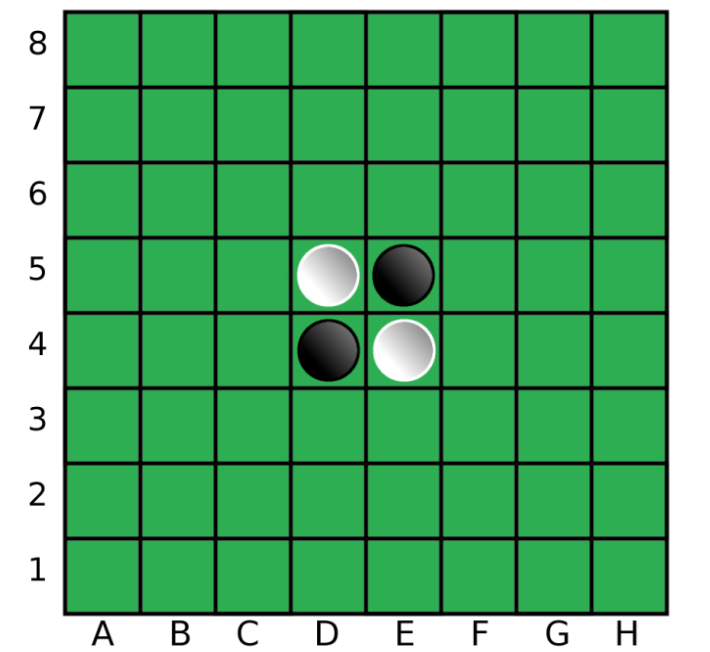
\includegraphics[width=\textwidth]{images/othello3.png}
    \caption{Początkowe ustawienie pionów.}
  \end{minipage}
  \begin{minipage}{0.49\textwidth}
    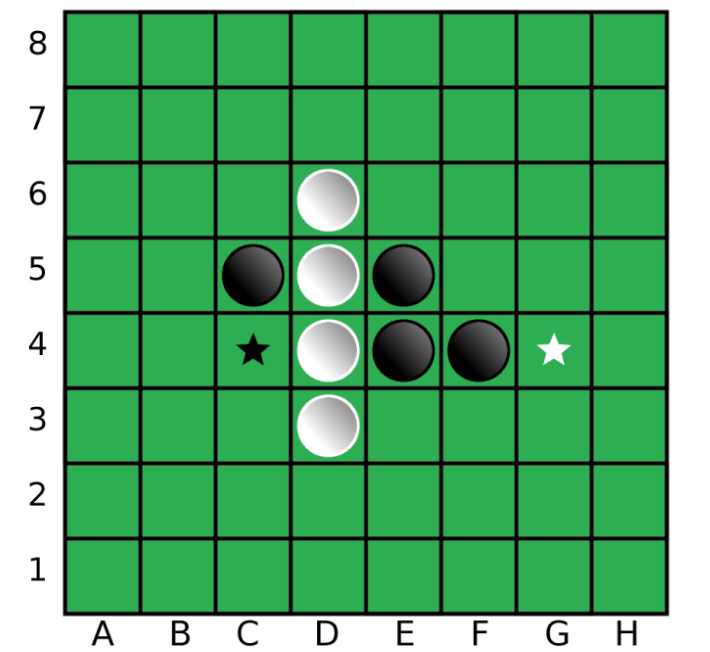
\includegraphics[width=\textwidth]{images/othello1.png}
    \caption{Diagram pokazujący przykładowe bicia.}
    \label{fig:bicia}
  \end{minipage}
\end{figure}
Rysunek \ref{fig:bicia} przedstawia możliwe bicia w danej sytuacji. Gdyby ruch miały czarne, mogłyby zagrać w pole zaznaczone czarną gwiazdką (C4). Wówczas pion stojący na polu D4 zostałby pojmany i zmieniłby kolor na czarny. W pojmaniu uczestniczyłby pion na polu E4.

Przejmowanie pionów jest obowiązkowe w każdym ruchu. Jeśli nie ma możliwości bicia,  to nie ma możliwości wykonania ruchu. Bicie jest możliwe w linii pionowej, poziomej i ukośnie. Jeśli w wyniku wykonania ruchu można bić w wielu kierunkach, bicie następuje we wszystkich kierunkach jednocześnie. Taką sytuację przedstawia diagram poniżej.

\begin{figure}[H]
\centering
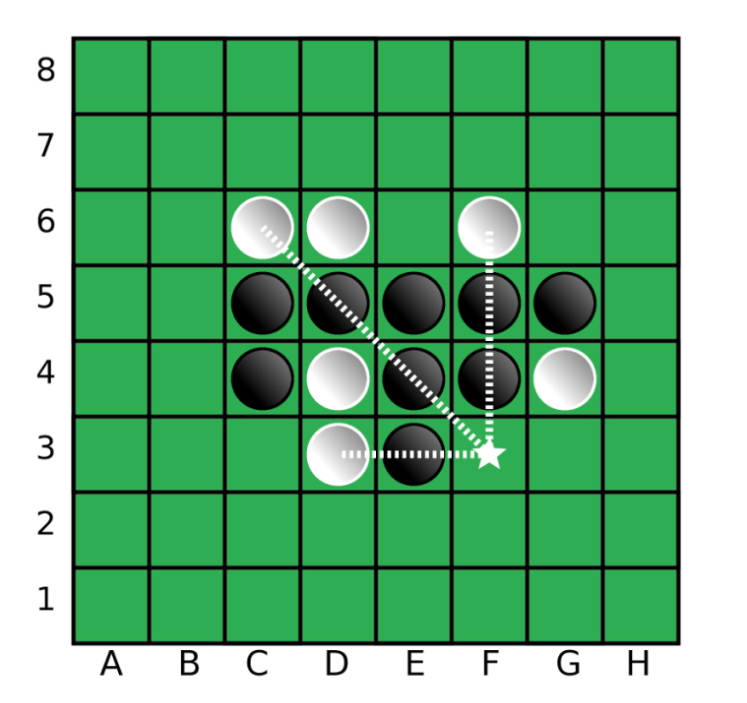
\includegraphics[width =0.5\columnwidth]{images/othello2.png}
\caption{Postawienie białego dysku na polu oznaczonym gwiazdką (F3) spowoduje bicie w pionie (pionów F4 i F5), w poziomie (piona E3) oraz ukośnie (piony E4 i D5). Wszystkie te piony zmienią po biciu kolor na biały.}
\end{figure}

Celem gry jest osiągnięcie maksymalnej liczby własnych pionów na planszy w momencie zakończenia gry. Gra kończy się, gdy wszystkie pola zostaną zajęte. W rzadkich sytuacjach może dojść do zakończenia gry wcześniej, jeśli żaden z graczy nie może wykonać żadnego ruchu. Najczęściej do takiej sytuacji dochodzi, gdy z planszy znikną wszystkie piony jednego gracza.

Może też dojść do sytuacji, gdy gracz nie może wykonać ruchu, ale jego przeciwnik tak. W takiej sytuacji gracz niemogący wykonać ruchu pasuje (traci kolejkę). Wykonuje następny ruch dopiero wtedy, gdy będzie miał taką możliwość.

\subsection{Monte Carlo Tree Search (MCTS)}
\label{sec:mcts}
\textbf{Monte Carlo Tree Search (MCTS)} jest metodą podejmowania decyzji o wyborze danej akcji w pewnym stanie. Jest ona szeroko używana do tworzenia sztucznych inteligencji zajmujących się graniem w gry dwuosobowe. Znajduje ona swoje zastosowanie przy tworzeniu drzewa gry, opisującego jakość kolejnych ruchów możliwych do wykonania w danych pozycjach.

W metodzie tej, drzewo gry budowane jest asymetrycznie, w kierunku najbardziej obiecujących ruchów. Należy przez to rozumieć ruchy, które przynosiły najlepsze rezultaty dla przeprowadzonych symulacji. Działanie metody można podzielić na etapy, które wykonywane są w każdej iteracji budowy drzewa:
\begin{enumerate}
    \item Selekcji - rozpoczynając od korzenia drzewa, odpowiadającego stanowi startowemu, wybierane są kolejne wierzchołki potomne (kolejne ruchy) aż do dotarcia do liścia drzewa. Sposób wyboru węzłów potomnych jest zależny od metody, ale ogólnie jego celem jest rozwijanie drzewa w kierunku najbardziej obiecujących ruchów.
    \item Ekspansji - jeśli wybrany ruch nie kończy gry to dla odpowiadającego mu węzła tworzone są jeden lub więcej węzłów potomnych i wybierz z nich jeden.
    \item Symulacji - rozgrywana jest losowa symulacja rozpoczynana w węźle wybranym w ekspansji.
    \item Propagacji wstecz (backpropagation) - na podstawie wyniku rozegranej symulacji uaktualniane są wierzchołki na ścieżce od korzenia do punktu wybranego w etapie ekspansji. To uaktualnienie brane jest pod uwagę przy selekcji w kolejnych iteracjach.
\end{enumerate}

\subsection{Upper Confidence Bound Applied To Trees (UCT)}
\label{sec:uct}
\textbf{UCT} jest najbardziej znanym i najszerzej stosowanym algorytmem mającym na celu ulepszenie procesu selekcji w metodzie MCTS. Jej celem jest znalezienie równowagi między podejściem dążącym do eksploatacji obecnie najlepszego rozwiązania oraz eksploracji w poszukiwaniu innych, potencjalnie lepszych rozwiązań. Algorytm UCT powstał na bazie innego rozwiązania - \textbf{Upper Confidence Bound (UCB1)}, przenosząc jego logikę na drzewa. Akcja wybierana w określonym położeniu jest definiowana za pomocą następującego wzoru:
\begin{equation}\label{eq:uct}
    a^* = arg max_{a \in A(s)} \left\{ Q(s,a) + C \sqrt{\frac{ln[N(s)]}{N(s,a)}} \right\}
\end{equation}
Gdzie $a$ oznacza akcję, $s$ to obecny stan, $A(s)$ jest zbiorem akcji możliwych do wykonania w stanie $s$, $Q(s,a)$ to ocena jakościowa akcji $a$ wykonanej w stanie $s$, $N(s)$ oznacza liczbę poprzednich wizyt algorytmu w stanie $s$, $N(s,a)$ to liczba to liczba tych wizyt zakończonych wyborem akcji $a$, zaś $C$ to współczynnik definiujący jak duży wpływ na wybór wyniku ma eksploracja (może być rozumiany jako \textquote{ciekawość} algorytmu). Na potrzeby tego badania, zgodnie z popularną praktyką, przyjęto $C = \sqrt{2}$.

\subsection{Usprawnienia UCT}
W ramach badań, podstawowa wersja metody MCTS z algorytmem UCT została porównana z dwoma jej ulepszeniami oraz klasycznym podejściem heurystycznym. Obie modyfikacje zaczerpnięte zostały z literatury. Ich opis przedstawiają sekcje \ref{sec:ucb1-tuned} oraz \ref{sec:mod2}

\subsubsection{UCB1-tuned}
\label{sec:ucb1-tuned}
Bezpośrednim skutkiem powiązań między algorytmem UCT oraz UCB (wspomnianym w sekcji \ref{sec:uct}) jest dokładne przeniesienie modyfikacji UCB na implementowany algorytm UCT. Jednym z takich ulepszeń jest algorytm \textbf{UCB1-tuned}. Modyfikacja ta skupia się na \textquote{ciekawości} algorytmu określanej wartością parametru $C$, występującego we wzorze \ref{eq:uct}. Stała wartość jest w tym przypadku zastąpiona wartością określoną za pomocą wzorów \ref{eq:ucb1-c} oraz \ref{eq:ucb1-v}:
\begin{equation}\label{eq:ucb1-c}
    C = \sqrt{min\left\{ \frac{1}{4}, V_i(n_i) \right\}}
\end{equation}

\begin{equation}\label{eq:ucb1-v}
    V_i(n_i) = \left(  \frac{1}{n_i} \sum_{m=1}^{n_i} X_{i,m}^{2} \right) - \overline{X_{i,n_i}}^{2} + \sqrt{\frac{2ln(n)}{n_i}}
\end{equation}

Intuicyjnie, modyfikacja ta powinna pozytywnie wpływać na jakość rozwiązania, poprzez lepsze dostosowanie wyborów algorytmu do obecnej sytuacji w drzewie gry.

\subsubsection{Transpozycje i grupowanie ruchów}
\label{sec:mod2}
Modyfikacja polega na zamianie drzewa na acykliczny graf skierowany, w którym znajdować się będą stany gry.
Z racji, że plansza do gry w Othello jest symetryczna, często może dochodzić do sytuacji w których jedna konfiguracja planszy może występować w drzewie gry więcej niż raz, lecz poddana obrotowi lub różniąca się tylko kolorami (tzn. jedna konfiguracja może być otrzymana \textquote{odwracając} kolory pionów oraz gracza wykonującego ruch w drugiej). Ponadto wiele konfiguracji może być osiągalnych za pomocą różnych sekwencji ruchu. W takim wypadku, jeżeli dla danej sytuacji w grze, w drzewie znajduje się już węzeł z analogiczną sytuacją, to zamiast dodawać do drzewa nowy węzeł jako potomka, w węźle rodzica umieszczany jest wskaźnik na węzeł już obecny w drzewie. Dzięki temu każdy stan gry jest umieszczany w drzewie tylko raz, a co za tym idzie statystyki dla losowych symulacji będą zbierane wspólnie i nie będą zależne od położenia węzła w drzewie. Powinno to nie tylko zmienić ilość węzłów w strukturze (która w sumie nie będzie już drzewem, a grafem), lecz także poprawić działanie dzięki współdzieleniu informacji o symulacjach.

\subsection{Podejście heurystyczne}
\label{sec:heuristic}
Zastosowane podejście heurystyczne opiera się na wykorzystaniu algorytmu \textit{alpha–beta pruning}. Algorytm ten używany jest często do przeszukiwania drzew gry, w szczególności w sytuacjach gdy znane jest całe drzewo. Dla takich przypadków, algorytm zawsze znajduje najlepsze rozwiązanie. Ponadto, w takich sytuacjach jest on szybszy od algorytmów takich jak \textit{backtracking}, dzięki wprowadzeniu ograniczeń oznaczanych przez $\alpha$ (\textit{alpha}) oraz $\beta$ (\textit{beta}), używanych do \textquote{obcinania} niektórych ścieżek, niepozwalających na uzyskanie lepszego rezultatu. W przypadku opisywanego zadania, skuteczność \textit{alpha–beta pruning} będzie zdecydowanie niższa, gdyż wygenerowanie i analiza niemal pełnego drzewa gry w Othello jest zadaniem zbyt czasochłonnym dla normalnych komputerów. Z tego też powodu zaimplementowany algorytm bada wyłącznie określoną ilość kolejnych poziomów drzewa gry, a w najniższym z nich pozycja oceniana jest z użyciem pomocniczej funkcji.

Wspomniana funkcja przyporządkowuje każdemu polu na planszy pewną wartość określoną przez oceną ekspertów i badaczy gry w Othello. Następnie, pozycja każdego gracza zostaje oceniona jako suma wartości z pól zajętych przez piony gracza w danej pozycji. Wyższa wartość tej funkcji oznacza lepszą (heurystycznie) pozycję. Wartości pól zdefiniowane są poprzez kwadratową macierz \texttt{WEIGHTS}, o wymiarach równych wymiarom planszy. Wartość funkcji dla pola o współrzędnych $i,j$ jest równa \texttt{WEIGHTS[i][j]}. Macierz z wagami przedstawiona jest na rysunku \ref{fig:weights}. Duże wartości w rogach planszy mają promować wybór tych pól, gdyż są one bezpieczne przed przejęciem.

\begin{figure}[H]
\centering
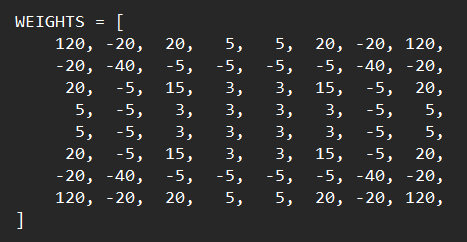
\includegraphics[width =0.5\columnwidth]{images/matrix.png}
\caption{Macierz wag pól na planszy.}
\label{fig:weights}
\end{figure}

\section{Przegląd literatury}
Artykułem, który był pomocny przy poszukiwaniach modyfikacji, był przegląd prac naukowych dotyczących Monte Carlo Tree Search: \textit{A Survey of Monte Carlo Tree Search Methods} \cite{review}. Był on między innymi uzupełnieniem informacji z wykładu dotyczących pierwszej modyfikacji czyli \textbf{UCB1}. Ponadto był inspiracją dla sformułowania drugiej modyfikacji.

Dodatkową pracą pomocną przy tworzeniu drugiej modyfikacji był artykuł \textit{Transpositions and move groups in Monte Carlo tree search
} \cite{transposition}.  Praca ta dokładniej opisuje zastosowanie skierowanych acyklicznych grafów  jako modyfikację UCT. Zaprezentowane w niej eksperymenty pokazują, że metoda ta może dać bardzo dobre rezultaty. Sformułowana modyfikacja łączy opisane w artykule idee transpozycji (możliwości różnych sekwencji ruchów do doprowadzenia do tej samej sytuacji) i grupowania ruchów (łączenia podobnych ruchów w jeden).

Dodatkowo przy opisie zasad gry Othello pomocny przydał się blog autorstwa Marcina Maja \textit{https://bonaludo.com/} \cite{Othello}, na którym opisane zostają różnice pomiędzy grami Othello i Reversi i zasady tej pierwszej.
\section{Hipotezy badawcze}
\begin{itemize}
    \item Podstawowa wersja MCTS pokonuj w bezpośredniej rywalizacji algorytm heurystyczny.
    \item Modyfikacja \nameref{sec:ucb1-tuned} jest w bezpośredniej rywalizacji lepsza niż podstawowa wersja MCTS oraz algorytm heurystyczny.
    \item Najlepsze efekty daje modyfikacja \nameref{sec:mod2}, pokonując wszystkie pozostałe wersje w rozgrywkach bezpośrednich.
    \item Heurystyczny algorytm jest pokonywany przez średnio-zaawansowanego gracza w znacznej większości pojedynków.
    \item Wszystkie implementacje oparte na bazie MCTS prezentują poziom podobny do średnio-zaawansowanego gracza. Oznacza to, że podobną część pojedynków wygrywają gracze oparci na SI oraz gracz prawdziwy.
\end{itemize}

\section{Eksperymenty}
Hipotezy zweryfikowane zostały poprzez przeprowadzenie dwóch rodzajów eksperymentów: bezpośrednich pojedynków między zaimplementowanymi SI oraz pojedynków między każdą z SI a średnio-zaawansowanym graczem.

\subsection{Bezpośrednie pojedynki}
Pierwszą częścią testów były mecze, w których ruchy obu graczy były wyznaczane przez zaimplementowane algorytmy. W stosunku do początkowych planów zmianie uległa jednak ilość spotkań rozgrywanych przez każdą parę algorytmów. Początkowo miały to być 2 bądź 3 spotkania, z losowym wyborem gracza rozpoczynającego rozgrywkę w 1 i 3 spotkaniu. Po przemyśleniu tego podejścia, uznano je jednak za błędne. W odróżnieniu od pojedynków między rzeczywistymi graczami, algorytmom nie robiło różnicy jakim kolorem pionów rozgrywane było pierwsze spotkanie. Ponadto, przy zadanym ziarnie generatora liczb pseudolosowych, wynik trzeciego spotkania był jednakowy z wynikiem jednego z poprzednich (w zależności od wylosowanych kolorów). Powodowało to wyłącznie niepożądane, losowe zaburzenie wyników. Reasumując, rozegrane zostały wyłącznie po 2 mecze (różnymi kolorami) w każdej parze algorytmów. Tego typu spotkania zostały następnie powtórzone dla 5 różnych ziaren generatorów liczb pseudolosowych. Każde wygrane spotkanie \textquote{nagradzane} było 1 punktem dla zwycięskiego algorytmu, zaś remis dawał po $0,5$ punktu obu graczom. Poniższa tabela \ref{tab:test1a} prezentuje podsumowanie rezultatów przeprowadzonych testów.

\begin{table}[H]
\centering
\begin{tabularx}{0.7\textwidth}{c|c|c|c|c|c}
\hline
Pozycja & Algorytm & Punkty & Zdobyte & Stracone & Bilans \\
\hline \hline
1 & MCTS podstawowe & \textbf{20,5} & 1062 & 856 & +206 \\
2 & MCTS z grupowaniem & \textbf{18,0} & 1038 & 882 & +156 \\
3 & MCTS z UCB1 & \textbf{12,0} & 908 & 1004 & -96 \\
4 & Heurystyka & \textbf{9,5} & 822 & 1088 & -266 \\
\hline
\end{tabularx}
\caption{Ranking algorytmów na podstawie przeprowadzonych testów}
\label{tab:test1a}
\end{table}

Wszystkie testy zostały przeprowadzone dla stałych wartości limitu poziomów analizowanych przez \textit{alpha-beta prunning} w algorytmie heurystycznym oraz liczby symulacji uruchamianych w \textit{MCTS}. Były to wartości odpowiednio $6$ oraz $300$. Wartości te zostały eksperymentalnie wybrane jako kompromis między poziomem gry a czasem działania algorytmów. Czasy działania były zresztą kolejnym badanym parametrem. W każdym spotkaniu, dla obu algorytmów, mierzony był sumaryczny czas wykorzystany przez dany algorytm na wybieranie kolejnych ruchów. Średnia względem wszystkich rozegranych przez dany algorytm spotkań uwzględniona została w tabeli \ref{tab:test1b} oraz na wykresie na rysunku \ref{fig:test1b}. Maszyna używana w testach wyposażona była w sześciordzeniowy i dwunastowątkowy procesor AMD Ryzen 3600 o taktowaniu $3.6 GHz$ oraz $48GB$ pamięci RAM o taktowaniu $3200 MHz$.

\begin{table}[H]
\centering
\begin{tabularx}{0.45\textwidth}{c|c}
\hline
Algorytm & Średni czas działania [s] \\
\hline \hline
MCTS podstawowe & 127,81 \\
MCTS z grupowaniem & 119,76 \\
MCTS z UCB1 & 125,02 \\
Heurystyka & 51,99 \\
\hline
\end{tabularx}
\caption{Średni czas działania algorytmów w przeprowadzonych testach}
\label{tab:test1b}
\end{table}

\begin{figure}[H]
\centering
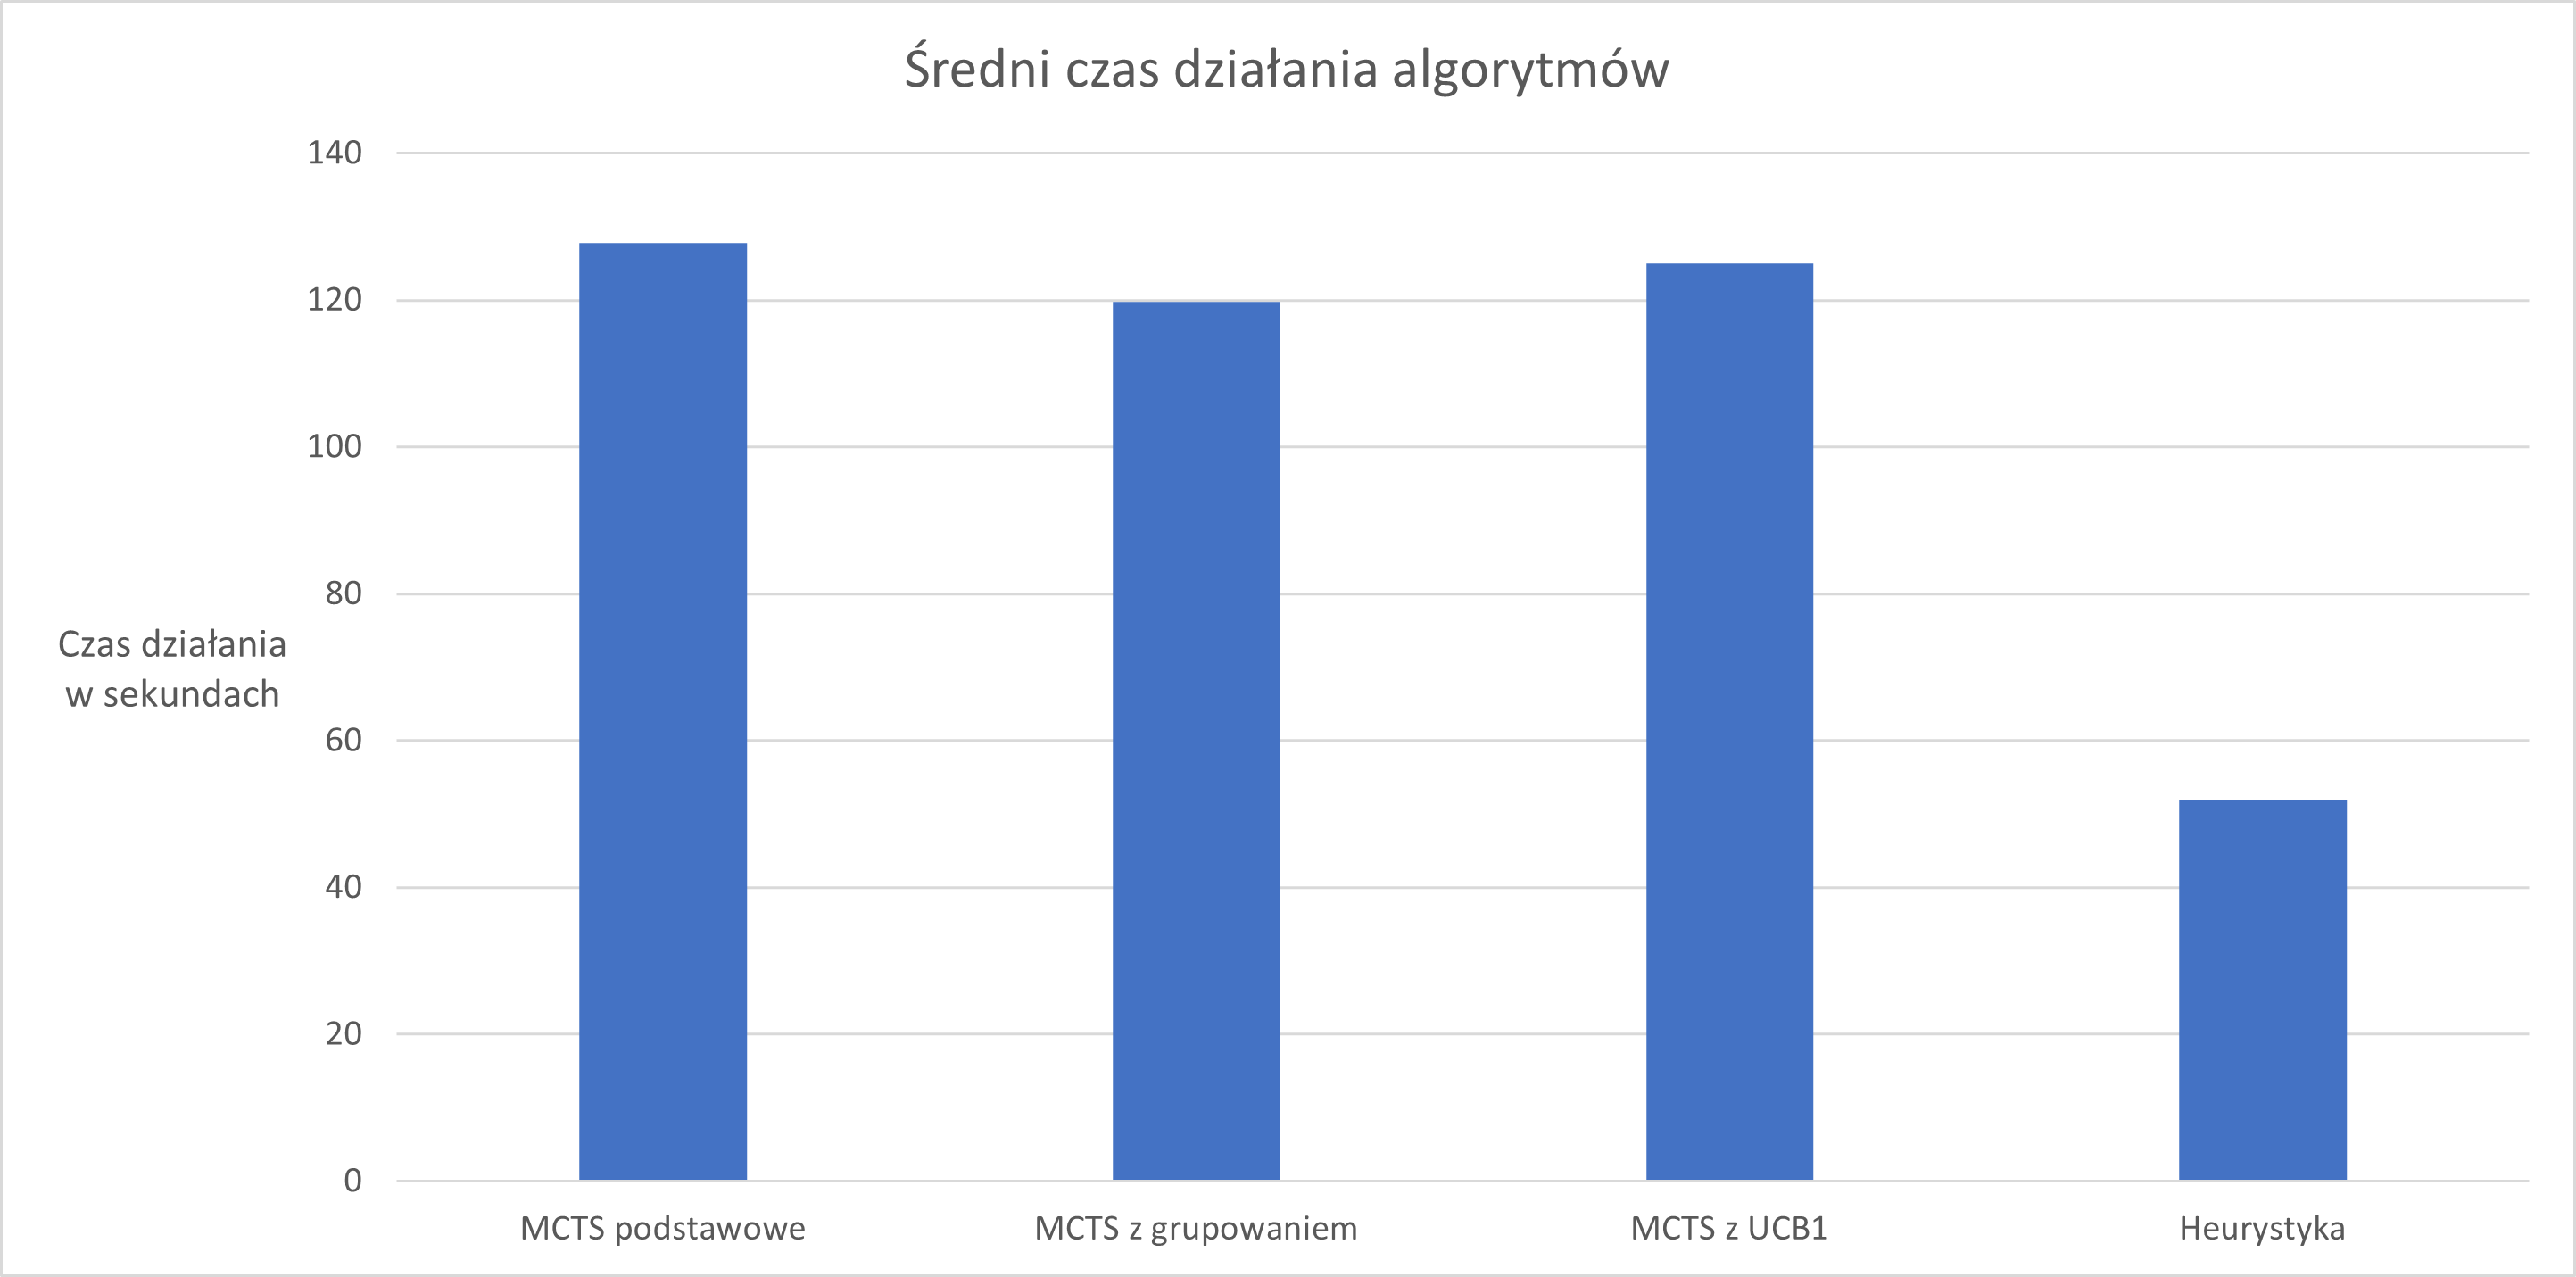
\includegraphics[width=\textwidth]{images/test1b.png}
\caption{Średni czas działania algorytmów}
\label{fig:test1b}
\end{figure}

Podsumowując wyniki testów, najlepszym algorytmem okazał się podstawowy algorytm \textit{Monte Carlo Tree Search} używający \textit{UCT}. Stan ten wynika ze sposobu implementacji, a w szczególności jednego z dodatkowych usprawnień wprowadzonych w algorytmie z grupowaniem. Aby wzmocnić główny cel wspomnianego ulepszenia, czyli poprawienie wydajności algorytmu, dodatkowo podjęto decyzję o zmniejszeniu liczby przeprowadzanych symulacji w pierwszej fazie gry. W teorii powinno to widocznie przyspieszyć działanie algorytmu, przy nieznacznym spadku jakości. Finalnie, przyspieszenie względem podstawowej wersji MCTS wyniosło średnio ok. 8 sekund (niecałe $6\%$), zaś rezultaty zmodyfikowanej wersji uplasowały ją na drugim miejscu rankingu.

Trzecie miejsce zajęła SI korzystająca z MCTS ulepszonego poprzez wykorzystanie \textit{UCB1}. Przeprowadzone testy poddały zatem pod wątpliwość sens implementacji tej bardziej skomplikowanej wersji. Przy pomijalnym zysku w kwestii czasu działania, osiągnięte zostały znacznie gorsze rezultaty.

Zgodnie z przewidywaniami, najgorsze rezultaty zanotował algorytm heurystyczny. Z drugiej strony, średni czas jego działania był ponad dwukrotnie krótszy niż w przypadku algorytmów wykorzystujących MCTS. Właściwość ta wynikała jednak z dobranych wartości parametrów. Analizowanie wyłącznie $6$ kolejnych kroków (przy ok. 60 ruchach w trakcie rozgrywki), znacznie okroiło możliwości algorytmu. Jednocześnie, zwiększenie wartości parametru do wartości $7$ zwiększało czasy testów kilkukrotnie, tak iż heurystyka potrzebowała widocznie więcej czasu niż pozostałe algorytmy. Z tego powodu, uznano użycie wartości parametru równej $6$ za bardziej reprezentacyjne.

Potencjalnym czynnikiem, który mógł wpływać na osiągane wyniki były kolory używanych pionów. W większości gier dwuosobowych, gracz rozpoczynający rozgrywkę (w Othello grający czarnymi) jest w pewnym stopniu faworyzowany. Z tego powodu wyniki meczów zostały także pogrupowane względem kolorów, co przedstawia tabela \ref{tab:test1c}. Osiągnięte rezultaty były jednak zbliżone, co przy nieznacznej liczbie testów, zawierających element losowości, uznano za zbyt małą podstawę do wyciągania wniosków dotyczących przewagi danego koloru. Co ciekawe, nieznacznie lepsze wyniki osiągał gracz biały, czyli wykonujący ruch jako drugi.

\begin{table}[H]
\centering
\begin{tabularx}{0.55\textwidth}{c|c|c|c|c|c}
\hline
Pozycja & Kolor & Punkty & Zdobyte & Stracone & Bilans \\
\hline \hline
1 & Biały & \textbf{32,5} & 1945 & 1885 & +60 \\
2 & Czarny & \textbf{27,5} & 1885 & 1945 & -60 \\
\hline
\end{tabularx}
\caption{Wyniki przeprowadzonych testów z podziałem na kolory}
\label{tab:test1c}
\end{table}

\subsection{Pojedynki z graczem}
Drugą częścią testów były pojedynki z prawdziwym graczem. W tym przypadku mecze rozgrywane były na analogicznych zasadach jak w części pierwszej, z tym że ruchy jednego z graczy zawsze były wyznaczane przez prawdziwego, średnio-zaawansowanego gracza. Testy te pozwoliły określić ogólną skuteczność zaimplementowanych algorytmów. Również w tej części rozegranych zostało kilka meczów, jednak z powodu ograniczeń czasowych, ich ilość była znacznie mniejsza niż w poprzednim etapie. Dodatkowo, zbyt duża ilość meczów testowych mogłaby doprowadzić, że znudzony ludzki gracz wykonywałby ruchy szybko, bez odpowiedniego przemyślenia. W związku z tym, gracz rozegrał 3 mecze BO3 (\textit{Best of 3}, do 2 zwycięstw) z każdym botem. Wszystkie parametry testów były takie same jak w przypadku pojedynków botów z botami.

Wyniki przedstawione zostały w tabeli \ref{tab:test_user}. Można zauważyć na niej, że algorytm heurystyczny, podobnie jak w pojedynkach z innymi algorytmami, sprawił się ewidentnie najgorzej i nie był w stanie wygrać żadnej rundy. Nieco lepiej sprawiło się usprawnienie UCB1-tuned, gdyż było ono w stanie wygrać jedno BO3. Podstawowa wersja UCT sprawiła się nieznacznie lepiej od wersji z wykorzystanym grupowaniem, gdyż pomimo że obie wersje wygrały 2 BO3 i zremisowały jedno, to podstawowa wersja odniosła jedno zwycięstwo 2-0. Znaczna przewaga algorytmu UCT jest o tyle imponująca, że gry z nim były rozgrywane pod koniec testów, a poziom gracza stawał coraz lepszy z każdym meczem. Patrząc na podział punktów na kolory przedstawiony w tabeli \ref{tab:test_user_color}, można zauważyć zdecydowanie większą przewagę dla białego koloru niż dla pojedynków pomiędzy sztucznymi inteligencjami.

\begin{table}[H]
\centering
\begin{tabularx}{0.7\textwidth}{c|c|c|c|c|c}
\hline
Pozycja & Algorytm & Punkty & Zdobyte & Stracone & Bilans \\
\hline \hline
1 & MCTS podstawowe & \textbf{5,5} & 316 & 196 & +120 \\
2 & MCTS z grupowaniem & \textbf{5,5} & 294 & 282 & +12 \\
3 & MCTS z UCB1 & \textbf{3} & 226 & 286 & -60\\
4 & Heurystyka & \textbf{0} & 102 & 282 & -180 \\
\hline
\end{tabularx}
\caption{Ranking algorytmów na podstawie przeprowadzonych pojedynków z ludzkim graczem}
\label{tab:test_user}
\end{table}

\begin{table}[H]
\centering
\begin{tabularx}{0.55\textwidth}{c|c|c|c|c|c}
\hline
Pozycja & Kolor & Punkty & Zdobyte & Stracone & Bilans \\
\hline \hline
1 & Biały & \textbf{19} & 1056 & 928 & +128 \\
2 & Czarny & \textbf{12} & 928 & 1056 & -128 \\
\hline
\end{tabularx}
\caption{Wyniki przeprowadzonych pojedynków botów z graczem z podziałem na kolory}
\label{tab:test_user_color}
\end{table}
\subsection{Sposób gry sztucznej inteligencji}
Tak jak wspomniano, algorytm UCT nie przegrał żadnego z 3 BO3 rozegranych z prawdziwym graczem. Warto jednak pochylić się nad tym, w jaki sposób sztuczna inteligencja jest w stanie osiągać tak dobry wynik. Podczas większości pojedynków, ludzki gracz do bardzo późnego etapu gry utrzymywał przewagę posiadanych dysków. Jednakże, w Othello sytuacja może ulec zmianie bardzo szybko i nawet przewaga ponad 20 pionków może zostać stracona w kilka ruchów. W wielu grach, gdy dochodziły one do finalnej fazy, pomimo dużej przewagi punktów graczowi zaczynało brakować ruchów dających mu więcej niż jedno przejęcie. Z kolei sztuczna inteligencja posiadała wiele ruchów przejmujących ok 8-10 dysków. Dzięki temu była ona w stanie szybko przechylić szale zwycięstwa na swoją stronę. Przykład takiej sytuacji w grze został przedstawiony na  rysunkach \ref{fig:strategia_uct1} i \ref{fig:strategia_uct2}. Liczby widoczne na polach oznaczają ile pól zostanie przejętych przy umieszczeniu piona na tym polu. Na przedstawionych rysunkach gracz grał czarnymi dyskami, a algorytm UCT białymi. Patrząc na dostępne ruchy, można łatwo zauważyć, że gracz miał ich dostępnych zdecydowanie mniej. Inną obserwacją, co prawda niewidoczną na wspomnianych rysunkach, jest fakt, że algorytm UCT nie zawsze skupiał się na przejmowaniu pól w rogach. Dało się również znacznie zauważyć, że sztuczna inteligencja nawet posiadając możliwość przejęcia bardzo korzystnych pól, odwlekała to w czasie, jeśli wiedziała, że gracz nie jest w stanie ich przejęć. Dzięki temu bardzo skutecznie zawężała ilość możliwych do dokonania przez gracza ruchów (na rysunku \ref{fig:strategia_uct1} można to zauważyć na nieprzejętym polu oznaczonym białym 6).
\begin{figure}[H]
  \centering
  \begin{minipage}{0.49\textwidth}
    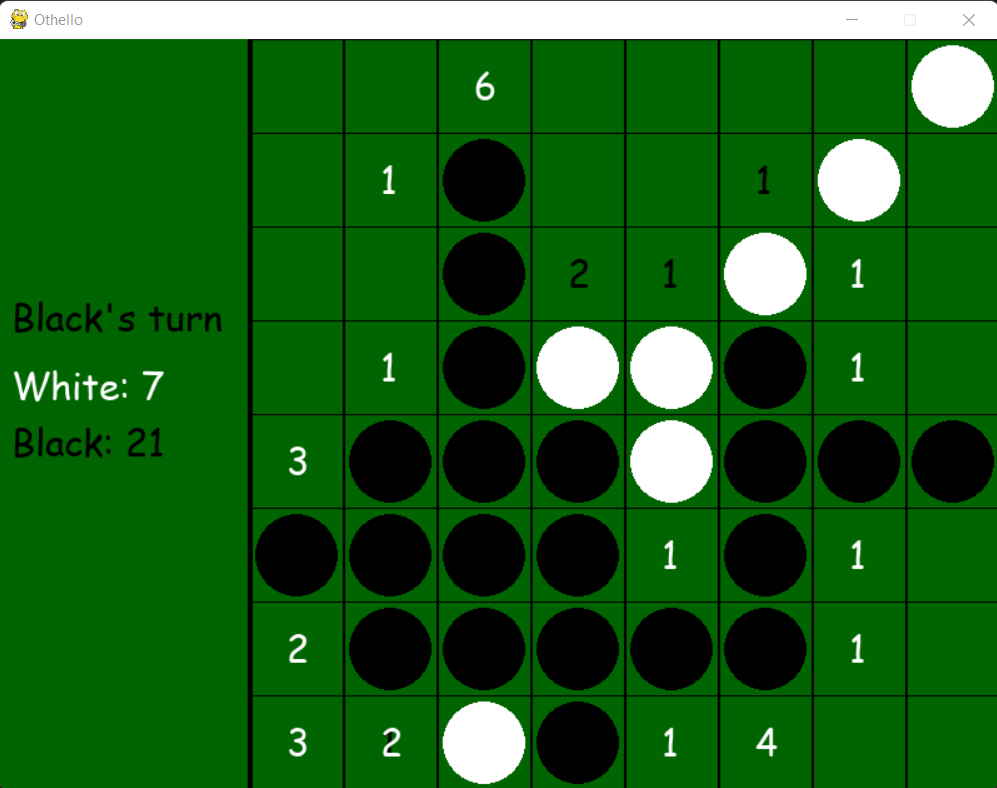
\includegraphics[width=\textwidth]{images/UCT_win_before.png}
    \caption{Sytuacja we wczesnej fazie gry.}
    \label{fig:strategia_uct1}

  \end{minipage}
  \begin{minipage}{0.49\textwidth}
    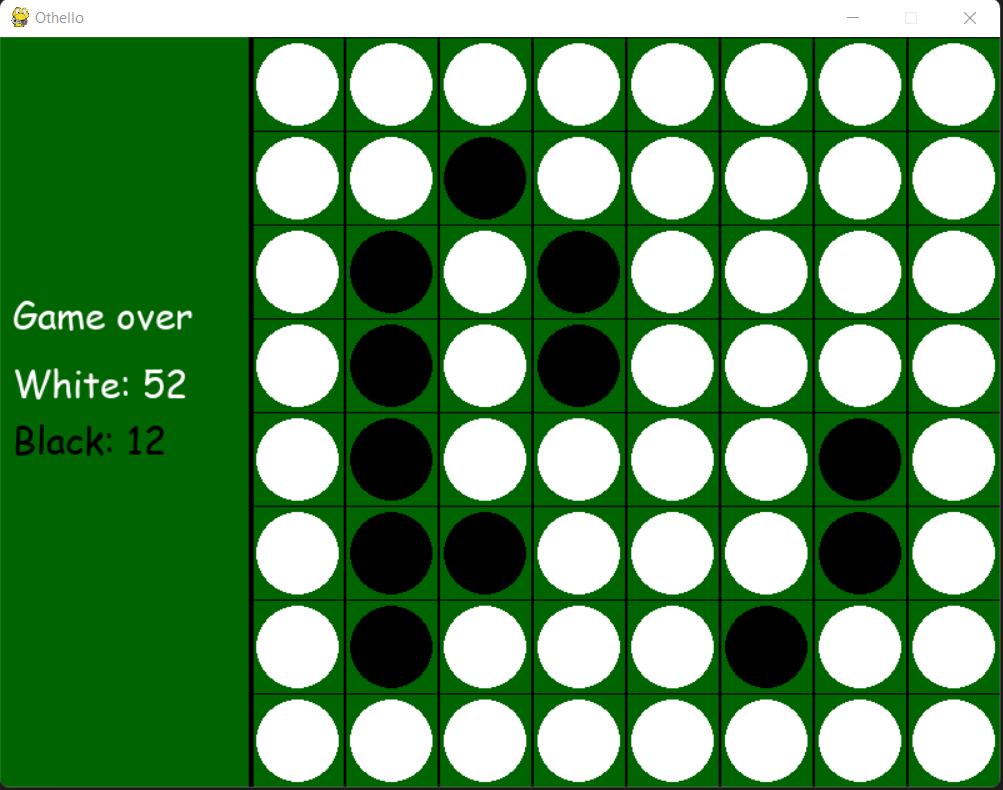
\includegraphics[width=\textwidth]{images/uct_win_after.png}
    \caption{Sytuacja w chwili zakończenia gry.}
    \label{fig:strategia_uct2}
  \end{minipage}
\end{figure}

\section{Implementacja}
Projekt został zaimplementowany przy użyciu języka \textit{Python}, wykorzystując biblioteki \textit{numpy}, \textit{math}, \textit{random} a także \textit{sys} oraz \textit{timeit}.

Gra udostępnia interfejs graficzny umożliwiający rozgrywkę pomiędzy dwoma graczami, gdzie każdy z nich może być sterowany przez jeden z zaimplementowanych algorytmów bądź przez użytkownika. Konfiguracja rozgrywki odbywa się w oparciu o plik konfiguracyjny w formacie JSON. Do stworzenia interfejsu graficznego wykorzystana została biblioteka \textit{pygame}.

\subsection{Konfiguracja}
W celu skonfigurowania rozgrywki, należy dokonywać zmian w pliku \textit{config.json}, umieszczonym w jednym katalogu z głównym skryptem. Plik konfiguracyjny powinien zostać stworzony w zgodzie z opisem w formacie \textit{schema}, zawartym w pliku \textit{config-schema.json}. Ponadto, szczegółowy opis parametrów konfiguracyjnych przedstawiono poniżej.
\begin{itemize}
    \item \textit{game\_type} - typ gry: \textquote{match} dla pojedynczej gry między dwoma graczami lub \textquote{tournament} dla turnieju BO3 rozgrywanego między wszystkimi graczami na zasadzie każdy z każdym.
    \item \textit{game\_repetitions} - opcjonalny (domyślnie: 1) parametr, określający ile razy testy powinny zostać powtórzone (dla różnych ziaren generatora liczb pseudolosowych).
    \item \textit{seed} - opcjonalny parametr, inicjujący generator liczb pseudolosowych, który następnie generuje kolejne ziarna dla kolejnych powtórzeń gry.
    \item \textit{heuristic\_simulation\_depth} - opcjonalny parametr (domyślnie 6), określający ile kolejnych poziomów powinien analizować \textit{alpha-beta pruning}.
    \item \textit{mcts\_simulation\_count} - opcjonalny parametr (domyślnie 300), określający ile symulacji powinno być przeprowadzonych w algorytmach bazujących na MCTS.
    \item \textit{show\_visualisation} - opcjonalny parametr (domyślnie \textit{true}), określający czy powinno zostać otworzone okienko z wizualzacją przebiegu gry. Ignorowane jeśli któryś z graczy jest człowiekiem (wtedy wizualizacja jest pokazywana zawsze).
    \item \textit{output\_file} - opcjonalny parametr zawierający ścieżkę do pliku wyjściowego z rezultatami kolejnych gier.
    \item \textit{players} - tablica zawierająca obiekty opisujące kolejnych graczy, z których każdy ma maksymalnie dwa atrybuty:
    \begin{itemize}
        \item \textit{player\_type} - algorytm używany do symulacji ruchów, lub \textquote{user} dla realnego gracza. Dopuszczalne wartości: \textquote{user}, \textquote{simple\_heuristic} (wyłącznie ocena najbliższego ruchu na podstawie funkcji heurystycznej z sekcji \ref{sec:heuristic}), \textquote{heuristic}, \textquote{random} (losowe dopuszczalne ruchy), \textquote{mcts\_uct}, \textquote{mcts\_ucb1}, \textquote{mcts\_grouping}.
        \item \textit{player\_color} - opcjonalny parametr określający kolor pionów gracza (\textquote{black} lub \textquote{white}). Parametr ignorowany dla trybu turniejowego lub gdy nie jest określony dla wszystkich graczy w spotkaniu.
    \end{itemize}
\end{itemize}

\section{Podsumowanie}
W wyniku przeprowadzonych testów, udało się, z różnymi wynikiami, zweryfikować prawdziwość postawionych hipotez. Zgodnie z oczekiwaniami, podstawowa wersja MCTS pokonała w bezpośredniej rywalizacji algorytm heurystyczny, który okazał się najgorszy spośród zaimplementowanych algorytmów.

Z kolei wbrew oczekiwaniom zaprezentowały się przedstawione modyfikacje MCTS. Obie osiągnęły rezultaty gorsze niż podstawowa wersja. Jednocześnie, na korzyść ulepszenia z transpozycją i grupowaniem ruchów można zaliczyć nieznaczne przyspieszenie tego algorytmu względem wersji podstawowej.

Porównanie algorytmów z żywym graczem również pozwoliło na potwierdzenie hipotez. Zgodnie z oczekiwaniami, algorytm heurystyczny okazał się gorszy od średnio-zaawansowanego gracza w każdym pojedynku. Z nawiązką została za to potwierdzona hipoteza dotycząca rezultatów MCTS w pojedynkach z graczem. O ile najgorszy wariant (tj. usprawnienie przez wykorzystanie UCB1-tuned) prezentował poziom porównywalny z graczem, to pozostałe modyfikacje znacząco go przewyższały, wygrywając w każdym pojedynku.

Innym aspektem, który nie został początkowo uwzględniony, jednak w wyniku testów okazał się potencjalnie interesującym do dalszej analizy, jest porównanie osiągnięć algorytmów w zależności od kolorów pionów. Przeprowadzone testy wskazują na nieznaczną przewagę osoby grającej pionami białymi. Ograniczony czas nie pozwolił jednak przebadać tego aspektu w sposób wystarczający do wyciągania wniosków.

\printbibliography

\end{document}